This section will explain the different tools and components used for the creation of the proyect.


%%%%%%%%%% 3D PRINTER %%%%%%%%%%%%%%%%%%%%%%%%%%%%%%%%%%%%%%%%%%%%%%%%%%%%%
\subsection{3D Printer}

	3D printers are Computer Numerical Control (CNC) machines that are capable of transforming virtual 3D models created with a Computer Aided Design (CAD) software into real-world objects.\\

	Created in 1984 by Chuck Hull of 3D Systems Corp this technology was little-known to the general public and was mainly used in industries for short runs of difficult pieces.\\
	In 2005 Dr. Adrian Bowyer, from the University of Bath, UK, started the RepRap project. Its goal was "to produce a pure self-replicating device not for its own sake, but rather to put in the hands of individuals anywhere on the planet, for a minimal outlay of capital, a desktop manufacturing system that would enable the individual to manufacture many of the artifacts used in everyday life" \\

	Today a vast range of 3D printers co-exist, varying in size, price and materials used. \\


	% $\rightarrow$ [RepRap, Zcorp, chocolate, liquid sint, micro, house building]\\

	% $\rightarrow$ [table with different methods?]\\

	In this theses a RepRap Prusa Air 2 (Figure \ref{tia}) model is used. It is of a "fused filament fabrication additive manufacturing" type. This type of printers extrude mainly ABS or PLA plastics, and deposit new liquified material over ther previous layer, now solid, effectively building parts from the bottom up layer by layer.\\

		\begin{figure}[H]
				\centering
				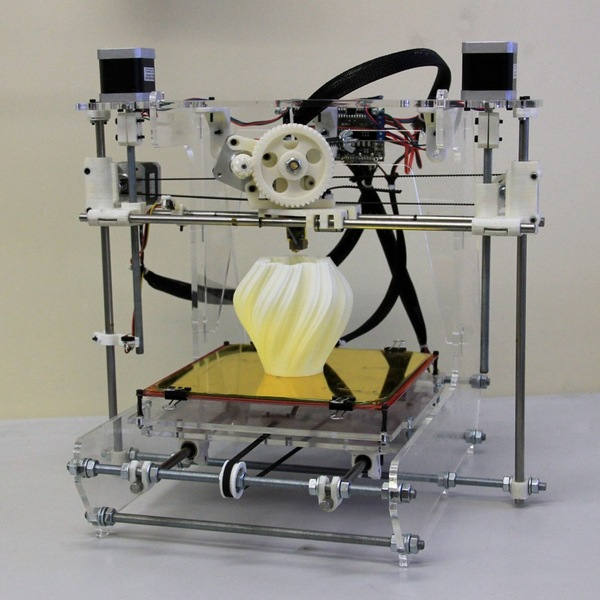
\includegraphics[scale=0.4]{images/ProjectComponents/tia.jpg}
				\caption{Prusa Air 2 3D printer}
				\label{tia}
			\end{figure}
			\bigskip














%%%%%%%%%% 3D SOFTWARE %%%%%%%%%%%%%%%%%%%%%%%%%%%%%%%%%%%%%%%%%%%%%%%%%%%%
\subsection{Software}
	This type of 3D printers work by turning 3D models into plastic parts. These models are first modelled in a CAD program and then processed with a \textit{slicing} software to divide the model into layers of G-code, which is the standard language interpreted by CNCs. This is then introduced into the printer to build the part.

		\subsubsection{3D Modelling }
		In this project SketchUp has been used to create the printed parts. Owned by the company Trimble Navigation it is a WYSIWYG (What You See Is What You Get) modelling editor with a large online warehouse of parts available for download. Figure \ref{sketchup} shows the program's user interface.\\

			\begin{figure}[H]
				\centering
				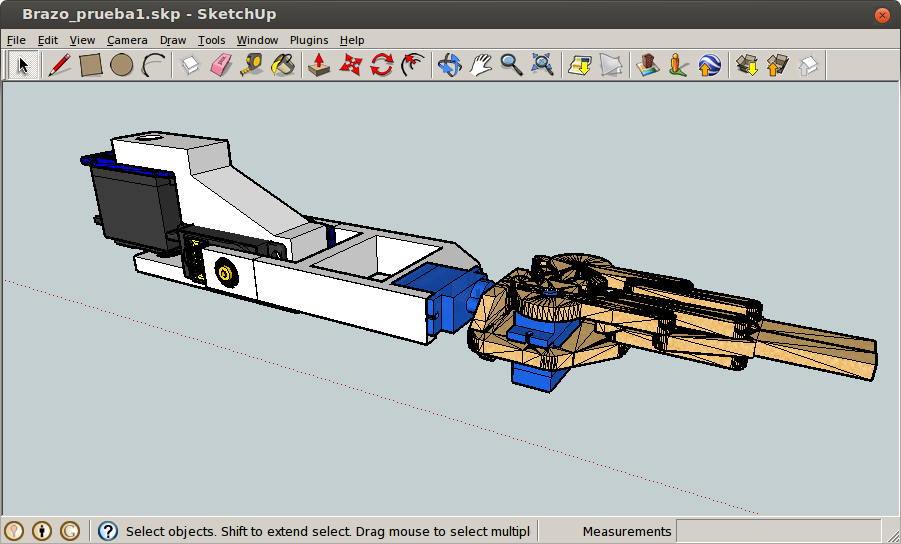
\includegraphics[scale=0.4]{images/ProjectComponents/sketchup-arm.png}
				\caption{SketchUp software}
				\label{sketchup}
			\end{figure}
			\bigskip

		In order to make it compatible with the slicing sofware, SketchUp's propietary format, \textit{SKP}, has to be converted to the standard \textit{STL}. In order to accomplish this the \textit{Su2stl.rb} plugin is installed. A new \textit{Plugins} menu appears in Sketchup which contains the Import/Export options, where the desired output format and model units are specified.



		\subsubsection{G-Code Generator} 
		Once the model is converted to \textit{STL} it then has to be sliced. Since 3D printers work by building layer upon layer of plastic, the model has to be transformed into the same format. The G-code generator converts the CAD model into layers of CNC instructions. There are three main slicing programs, each with their own benefits:

			\begin{itemize}
			  
			  \item Skeinforge: \hfill \\
			  The first slicing program used in homemade 3D printers. It is by far the most complete of the three. It allows the user to control each and every imaginable setting of the printer, from the axis' speeds to the retraction distance of the plastic into the extruder while moving. However, because of this it has a very steep learning curve which makes it unsuitable for the average consumer.

			  \item Slic3r:  \hfill \\
			  Slic3r was created as an user-friendly software, which only gives the final user a choice in the basic settings, such as printing speeds, filament widths or part infills. As a result it is an easier program to slice parts with a sufficient level of customization. It has nonetheless problems converting models with imperfections or broken shapes.
			  
			  \item Cura \hfill \\
			  Finally, Cura is also designed with user-friendliness in mind. This slicer is more robust than Slic3r, in that it will accept models with imperfections, and will try to correct them. It also features a box simulating the print area in which the model can be moved around, turned or scaled before printing.
			  This last feature is specially useful if minor changes need to be made, without returning to the CAD software.
			
			\end{itemize}

		To print the needed parts Cura was chosen because of its simplicity and usefulness in rearranging the objects without having to modify the original CAD files.


		\subsubsection{CNC Controller}
		Finally once the G-code is created it is passed on to a CNC controller which will feed all the code's commands to the printer. The chosen software, Pronterface (Figure \ref{pronterface}), allows the user to control the movement of the printer's axes, including the extruder, as well as the temperature settings or the calibration procedure.  


			\begin{figure}[H]
					\centering
					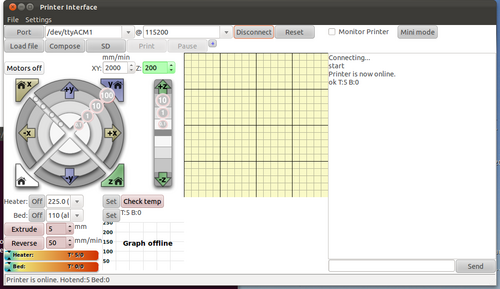
\includegraphics[scale=1.4]{images/ProjectComponents/pronterface.png}
					\caption{Pronterface CNC control software}
					\label{battery}
			\end{figure}
			\bigskip






%%%%%%%%%%%% BATTERY %%%%%%%%%%%%%%%%%%%%%%%%%%%%%%%%%%%%%%%%%%%%%%%%%%%%%%
\subsection{Li-Ion Battery}

	The whole system is powered by a lithium ion 12V 6800mAh battery as seen in Figure \ref{battery}. This was chosen because of the high voltage and durability it delivers over regular AA batteries.

		\begin{figure}[H]
				\centering
				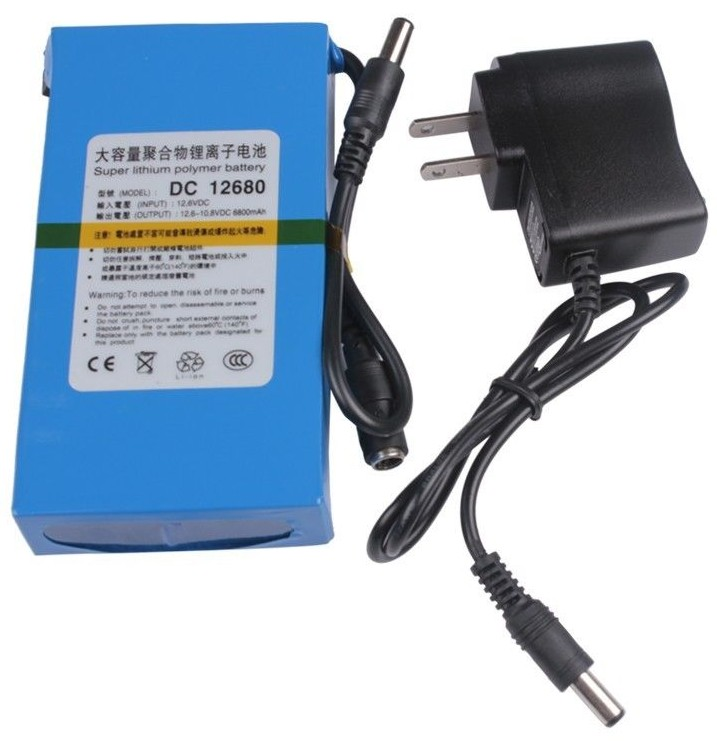
\includegraphics[scale=0.25]{images/ProjectComponents/battery.jpg}
				\caption{Li-ion 12V 6800mAh battery with charger}
				\label{battery}
		\end{figure}
		\bigskip

	











%%%%%%%%%%% CONVERTER %%%%%%%%%%%%%%%%%%%%%%%%%%%%%%%%%%%%%%%%%%%%%%%%%%%%%
\subsection{Voltage level converters}	

Different electronics demand different power levels, ranging from 3.3V up to 12V in this case. In order to provide suitable voltages to each part, different voltage level converters are used.

	\subsubsection{DC-DC Step-Down Converter}

		Voltage level converters are used to adapt a source's voltage to that required by the load. In this thesis a DC-DC converter is used to decrease the 12V given by the battery to the 5V required by the logic components as well as the servomotors. \\
		
		The simplest method would be to use a linear regulator such as a 7805, which is a cheap, single-component solution. However, this is greatly inefficient solution, since a great part of the power is dissipated as heat.
		For instance, if a 7805 were to be used in this project, about $\mathLarge{\frac{Power_{in} - Power_{out} }{Power_{in} }}=\mathLarge{\frac{12 \cdot I -5 \cdot I}{12\cdot I}}=\mathLarge{\frac{12-5}{12}}=58.33\%$ of the power is wasted.\\


		A much more efficient solution is to use a switching regulator such as a Buck converter, which has an efficiency level of around 95\%  \cite{buck}. 
		Buck converters work by switching rapidly between "On" and "Off" states, which sets the output voltage in function of the duty cycle $d=\mathLarge{\frac{time_{on}}{time_{on}+time_{off}}}$. The converter (Figure \ref{step-down}) used includes a potentiometer to set the output level by selecting the duty cycle. 
 
		

			\begin{figure}[H]
					\centering
					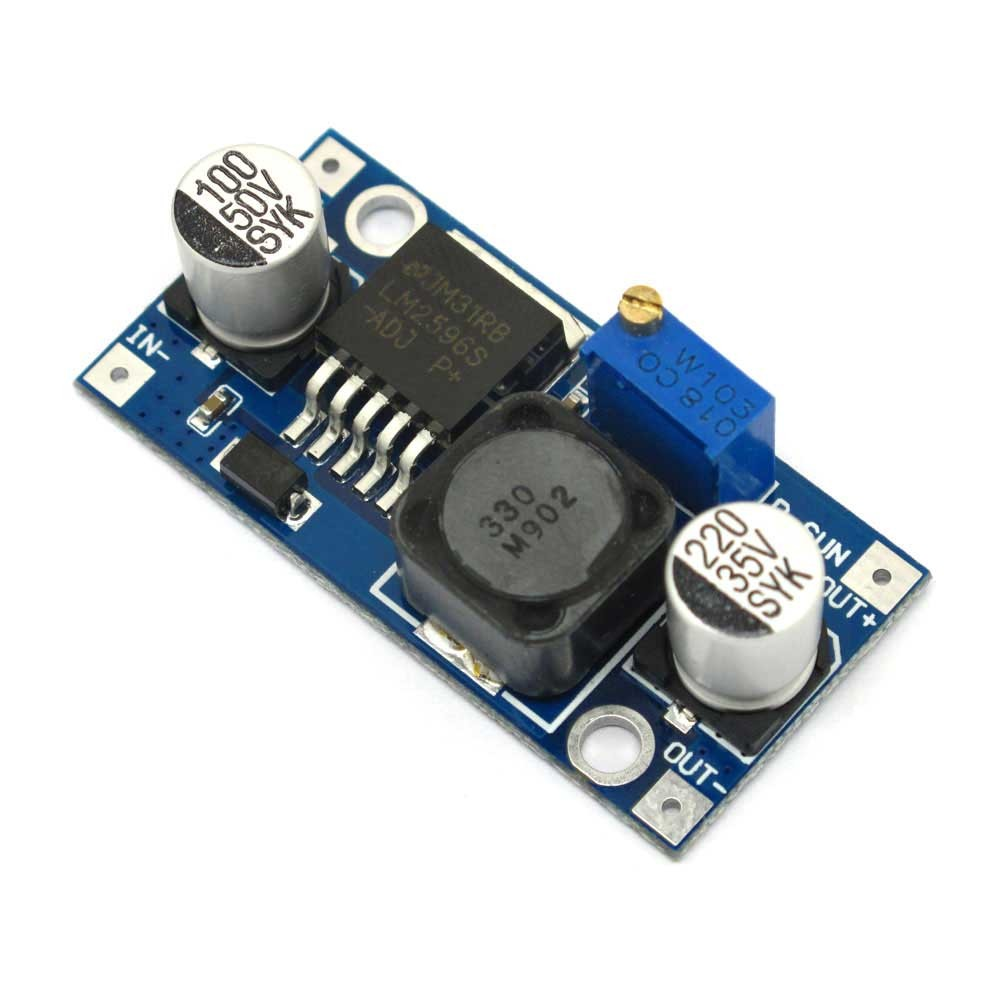
\includegraphics[scale=0.2]{images/ProjectComponents/buck.jpg}
					\caption{LM2596S step-down converter }
					\label{step-down}
			\end{figure}
			\bigskip

		The converter's electrical specifications are:
			\begin{itemize}
				\item Adjustable input voltage: 3.2 - 40V
				\item Adjustable output voltage: 1.25 - 35V ($V_{in} > V_{out}$ + 1.5V)       
				\item Max. output current: 3A
			\end{itemize}

	%\newpage
	\subsubsection{Bidirectional logic level converter}

		In order to enable serial communication between the Arduino and the Raspberry Pi another voltage level converter must be introduced, since the former operates at a 5V level while the latter does so at a 3.3V level.\\

		In this case a switching regulator like the previous one will not work because the communications are much faster than the regulator's switching speed. Therefore a bidirectinal, low power converter can be built out of transistors.\\

		Figure \ref{figure:levelShifter} shows a simple converter model.
		Analyzing the circuit from the low side: 
			\begin{itemize}
			\item If a logic one is emitted, the transistor source pin is grounded and it switches on, pulling down the high side to zero.
			\item If a logic zero is sent, the transistor is tied high and so is off, leaving the high pin connected to the pull-up resistor and thus seeing a one.
			\end{itemize}

			\begin{figure}[H]
					\centering
					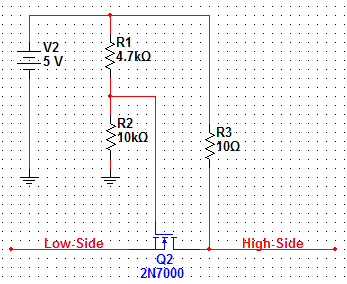
\includegraphics[scale=0.8]{images/ProjectComponents/level-converter-circuit.png}
					\caption{Bidirectional voltage converter}
					\label{figure:levelShifter}
			\end{figure}
			\bigskip

			This setup works for one line, two identical circuits are needed in order to provide for serial communication. For this project a commercial board (Figure \ref{level-converter}) is used to reduce the total size of the converter by using SMD components.

			\begin{figure}[H]
					\centering
					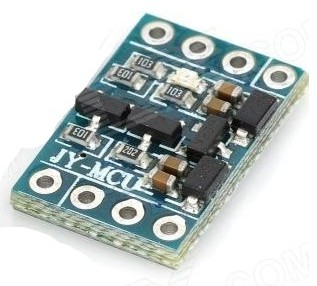
\includegraphics[scale=0.4]{images/ProjectComponents/logic-voltage.jpg}
					\caption{JY-MCU 5V-3V converter }
					\label{level-converter}
			\end{figure}
			\bigskip

		This board is used with UART communication, but is equally adequate for I$^2$C, SPI or one-wire communication.
 








\bigskip


%%%%%%%%%%% DC MOTORS %%%%%%%%%%%%%%%%%%%%%%%%%%%%%%%%%%%%%%%%%%%%%%%%%%%%%
\subsection{Motors}

Three different types of actuators are present in the robot, which are either continuous motors or servomotors.

	\subsubsection{DC motor}
	
	DC motors are simple actuators that start spinning whenever there is a voltage applied between their wires.  Their speed is directly dependent of the voltage level applied, and the turning sense on the polarity of the conection.\\

	This robot uses two GA25Y370-362 dc motors (Figure \ref{dc-motor}), which turn at a 10rpm with a torque of 5Nm when connected to a 12V source. 

		\begin{figure}[H]
			\centering
			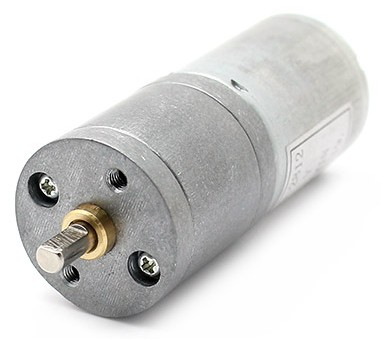
\includegraphics[scale=0.4]{images/ProjectComponents/motor.jpg}
			\caption{GA25Y370-362 motor }
			\label{dc-motor}
		\end{figure}
		\bigskip

	Since the motor only has two wires, a controller is needed to interface it to the arduino. This type of controller is called an H-bridge because of its circuit topology (Figure \ref{h-bridge}). It consists of a series of transistors that can be opened or closed to reverse the polarity of the motor, as well as to apply a PWM modulation to control its speed.\\

		\begin{figure}[H]
			\centering
			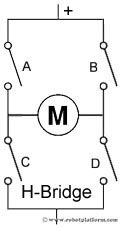
\includegraphics[scale=0.6]{images/ProjectComponents/h-bridge.jpg}
			\caption{H-bridge circuit }
			\label{h-bridge}
		\end{figure}
		\bigskip

	In this case a L293D chip with two internal H-bridge circuits is used to control both motors.

	\subsubsection{Servomotors}

	On the other hand, servomotors are much more complex than continuous motors. These consist of a regular dc motor, a set of gears, an internal potentiometer and a control circuit. They also do not revolve continuously but rather oscillate in a range of approximately 180º.	\\

	In order to control the servo the user gives the desired position through the input cable and the circuit board matches it to a resistance value. The motor then starts turning which does the same to the potentiometer, and stops when the latter reads the desired resistance value.\\

	The robot uses three GOTECK GS-551MG (Figure \ref{goteck}) servos per arm, which are used for the more demanding movements, while it employs two aditional TowerPro SG90 (Figure \ref{towerpro}) servos for the less challenging actions of wrist rotation and gripper manipulation.

		\begin{figure}[H]
			\centering
			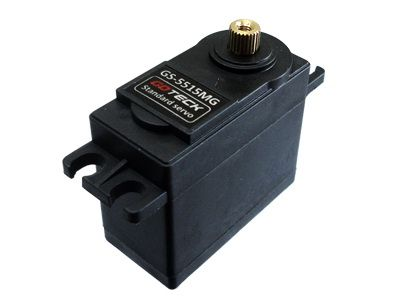
\includegraphics[scale=0.5]{images/ProjectComponents/servo1.jpg}
			\caption{GOTECK GS-551MG servo }
			\label{goteck}
		\end{figure}
		\bigskip

	The GOTECK's technical specifications are:
			\begin{itemize}
				\item Operating voltage: 4.8 V
				\item Maximum torque: 1.3 Nm    
				\item Speeed: 0.20sec/60deg
			\end{itemize}	

		\begin{figure}[H]
			\centering
			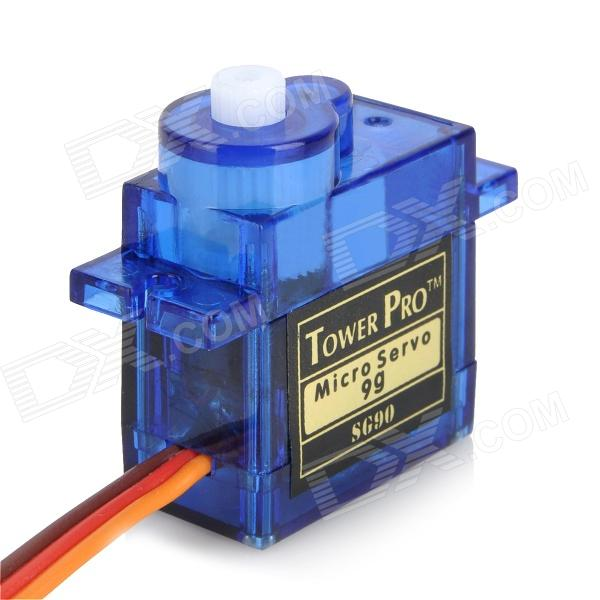
\includegraphics[scale=0.25]{images/ProjectComponents/servo2.jpg}
			\caption{TowerPro SG90 servo }
			\label{towerpro}
		\end{figure}
		\bigskip

	The TowerPro's technical specifications are:
			\begin{itemize}
				\item Operating voltage: 4.8 V
				\item Maximum torque: 0.18 Nm
				\item Speed: 0.10sec/60deg
			\end{itemize}	














%%%%%%%%%%%% ARDUINO %%%%%%%%%%%%%%%%%%%%%%%%%%%%%%%%%%%%%%%%%%%%%%%%%%%%%%
\newpage
\subsection{Arduino}

	Arduino is a family of low-cost electronic boards designed to be easily programmable. From the official Arduino website, "Arduino is an open-source electronics prototyping platform based on flexible, easy-to-use hardware and software. "\\

	Arduino is programmed using its own language, which is merely a set of C/C++ functions compiled with \textit{avr-g++}. They can nonetheless be programmed in pure C or C++ in an external IDE and have code uploaded to it as any other AVR board.\\

	In this proyect an Arduino Nano v3 with an ATmega 328 microcontroller has been chosen mainly due to its processing power and reduced size.
		
		\begin{figure}[H]
			\centering
			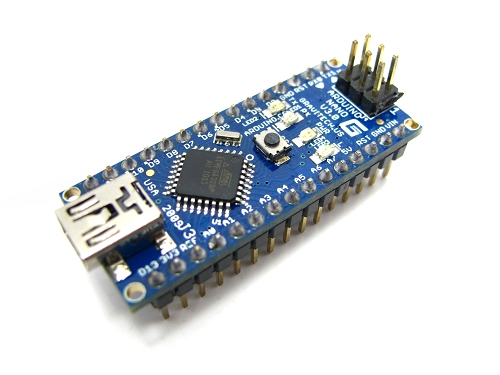
\includegraphics[scale=0.4]{images/ProjectComponents/arduino.jpg}
			\caption{Arduino Nano v3 }
			\label{}
		\end{figure}
		\bigskip

	The official Arduino Nano V3 specifications are:
		\begin{itemize}
			\item \textbf{Microcontroller:} Atmel ATmega168 or ATmega 328
			\item \textbf{Operating Voltage (logic level):} 5V
			\item \textbf{Input Voltage (recommended):} 7-12V
			\item \textbf{Input Voltage (limits):} 6-20V
			\item \textbf{Digital I/O Pins:} 14 (of which 6 provide PWM output)
			\item \textbf{Analog Input Pins:} 8
			\item \textbf{DC Current per I/O Pin:} 40mA
			\item \textbf{Flash Memory:} 16 KB (ATmega168) or 32 KB (ATmega328), of which 2 KB used by bootloader
			\item \textbf{SRAM:} 1 KB (ATmega168) or 2 KB (ATmega328)
			\item \textbf{EEPROM:} 512 bytes (ATmega168) or 1 KB (ATmega328)
			\item \textbf{Clock Speed:} 16MHz
			\item \textbf{Dimensions:} 0.73'' x 1.70''
			\item \textbf{Communications:} UART, SPI and I$^2$C buses
		\end{itemize}













%%%%%%%%%%% RASPBERRY %%%%%%%%%%%%%%%%%%%%%%%%%%%%%%%%%%%%%%%%%%%%%%%%%%%%%
\newpage
\subsection{Raspberry Pi}

	From the official website of the homonymous foundation, the Raspberry Pi is a "credit-card sized computer that plugs into your TV and a keyboard. It is a capable little computer which can be used in electronics projects."\\

		\begin{figure}[H]
				\centering
				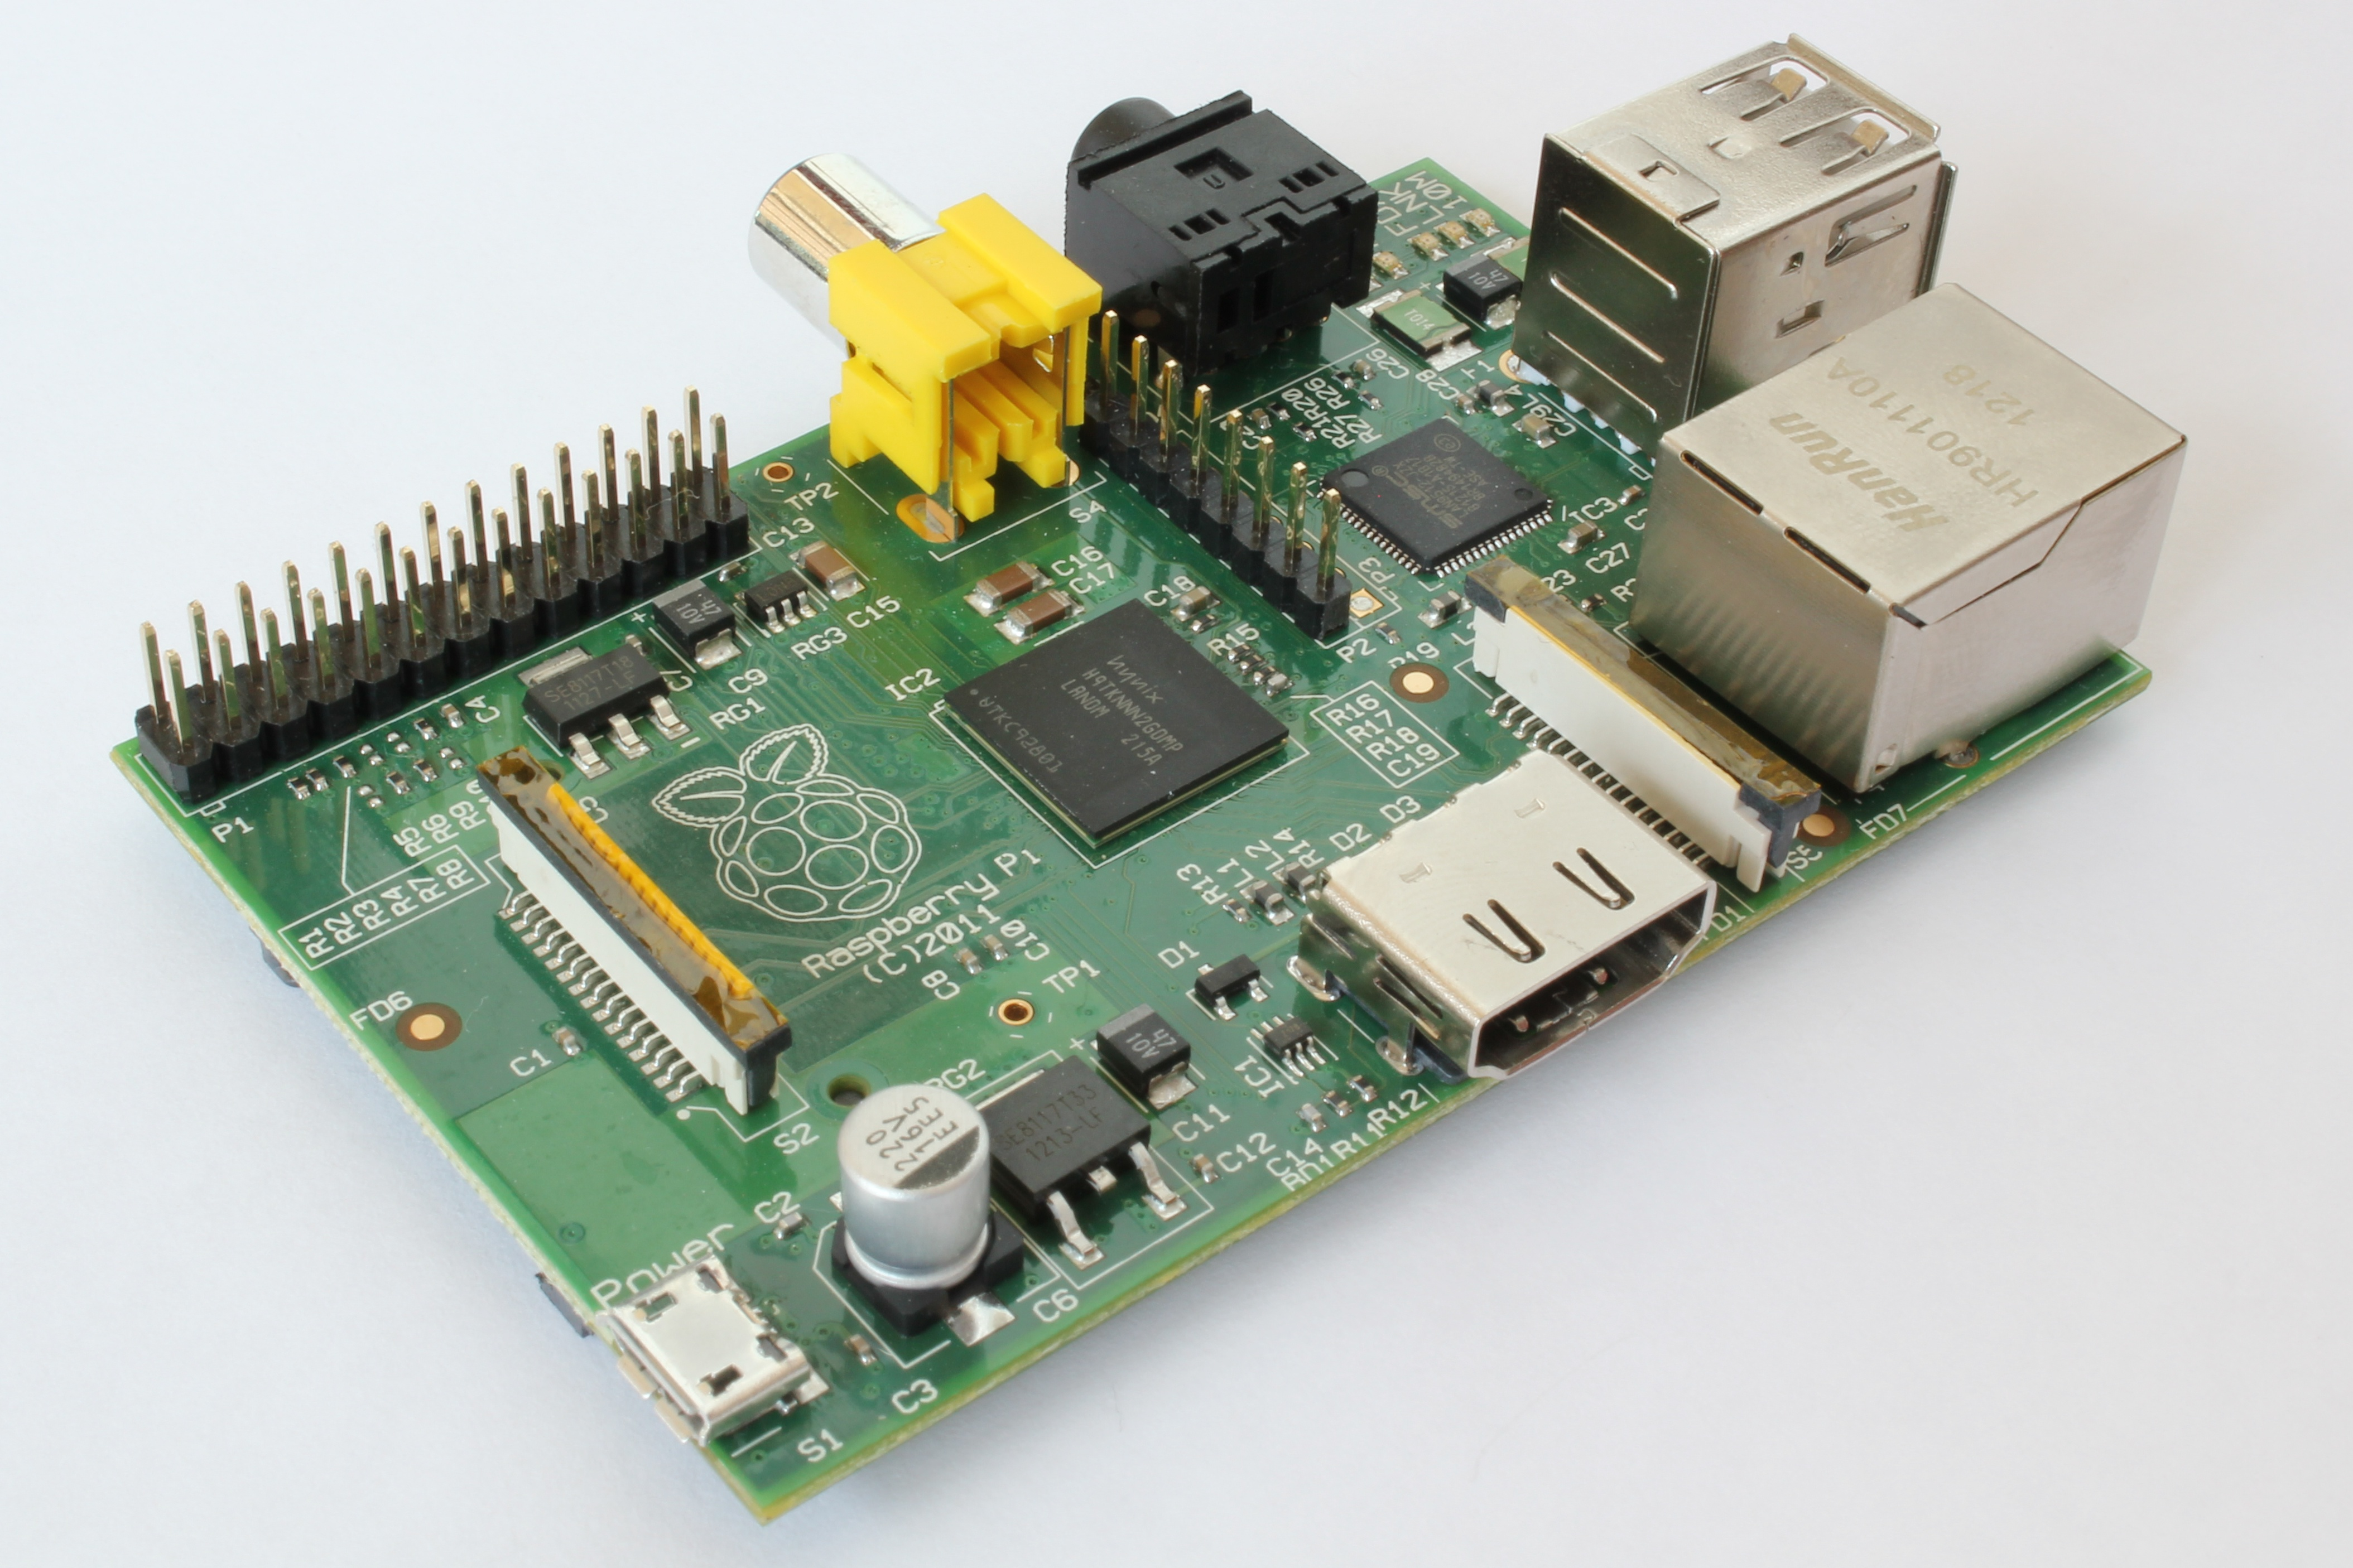
\includegraphics[scale=0.07]{images/ProjectComponents/raspberry.jpg}
				\caption{Raspberry Pi model B}
				\label{}
		\end{figure}
		\bigskip

	Available in two models, A and B, the Raspberry has a Broadcom BCM2835 System On a Chip, which includes an ARM1176JZF-S 700MHz processor and a VideoCore IV GPU. It includes as well a 256Mb RAM, upgraded to 512Mb in model B.\\

	\bigskip

	The Pi features: 
		\begin{itemize}
			  \item HDMI, composite and raw DSI video outputs
			  \item 3.5mm audio jack
			  \item SD card socket
			  \item Low-level peripheral connections including:
			  	\begin{itemize}
			  	\item 8 General Purpose Input Output (GPIO) pins
			  	\item Universal Asynchronous Receiver Transmitter (UART) bus
			  	\item Inter-Integrated Circuit (I$^2$C) bus
			  	\item 2 Serial Peripheral Interface (SPI) buses
			  	\item Power pins: 3.3V, 5V and GND
			  	\end{itemize}
			  \item Ethernet socket
			  \item USB hub (1 socket in model A, 2 in model B)

		\end{itemize}

	The main storage unit is the SD card, and that is where the OS is flashed, normally a Linux distribution. The most popular is Raspbian, an adapted version of Debian Wheezy, although other Linux distros or even other OS like Android or XBMC can be used.

		\begin{figure}[H]
		    \centering
		    \begin{subfigure}[b]{0.3\textwidth}
		        \centering
		        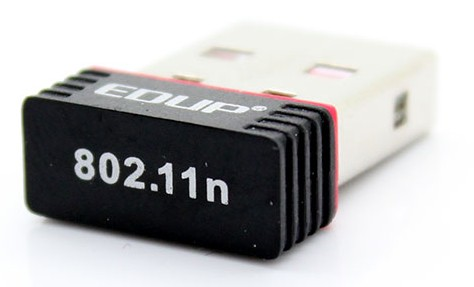
\includegraphics[scale=0.25]{images/ProjectComponents/wifi.jpg}
				\caption{WiFi USB dongle}
		        \label{}
		    \end{subfigure}
		    \hfill
		    \begin{subfigure}[b]{0.3\textwidth}
		        \centering
		        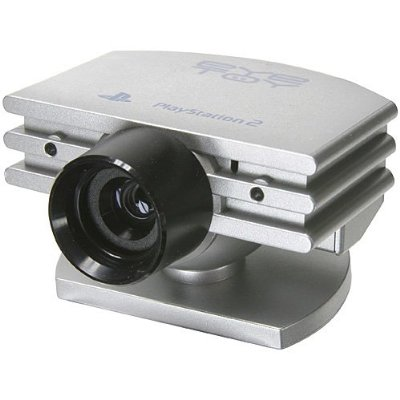
\includegraphics[scale=0.25]{images/ProjectComponents/camera.jpg}
				\caption{PlayStation 2 EyeToy }
		        \label{}
		    \end{subfigure}
		    \hfill
		    \begin{subfigure}[b]{0.3\textwidth}
		        \centering
		      	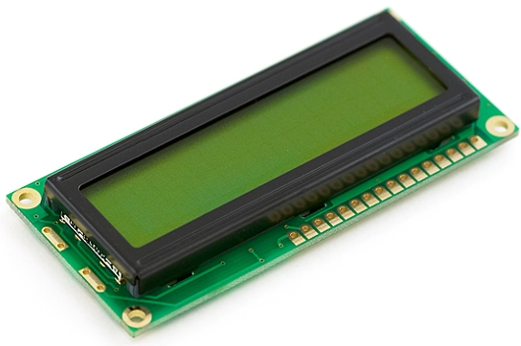
\includegraphics[scale=0.25]{images/ProjectComponents/lcd.jpg}
				\caption{LCD screen 16x2}
		        \label{}
		    \end{subfigure}
		    \caption{Raspberry Pi peripherals}
		    \label{}
		\end{figure}


	In this proyect a Raspberry Pi model B running Raspbian manages the software side of the robot. It has an Ralink Technologies RT5730 WiFi USB dongle , a PlayStation 2 EyeToy USB camera and a 16x2 character LCD screen connected in order to create a WIFI Access Point, stream video to the user and signal its status respectively.






%%%%%%%%%%% ANDROID %%%%%%%%%%%%%%%%%%%%%%%%%%%%%%%%%%%%%%%%%%%%%%%%%%%%%%%
\newpage
\subsection{Android Phone}

Android is one of the most popular operating systems for smartphones. Created in 2003 by the eponymous company and adquired by Google Inc. two years later, its open-source nature has incentivised manufacturers to include it in their products, expanding its reach until it has dominated the market share, as seen in Figure \ref{marketshare}.

	\begin{figure}[H]
			\centering
			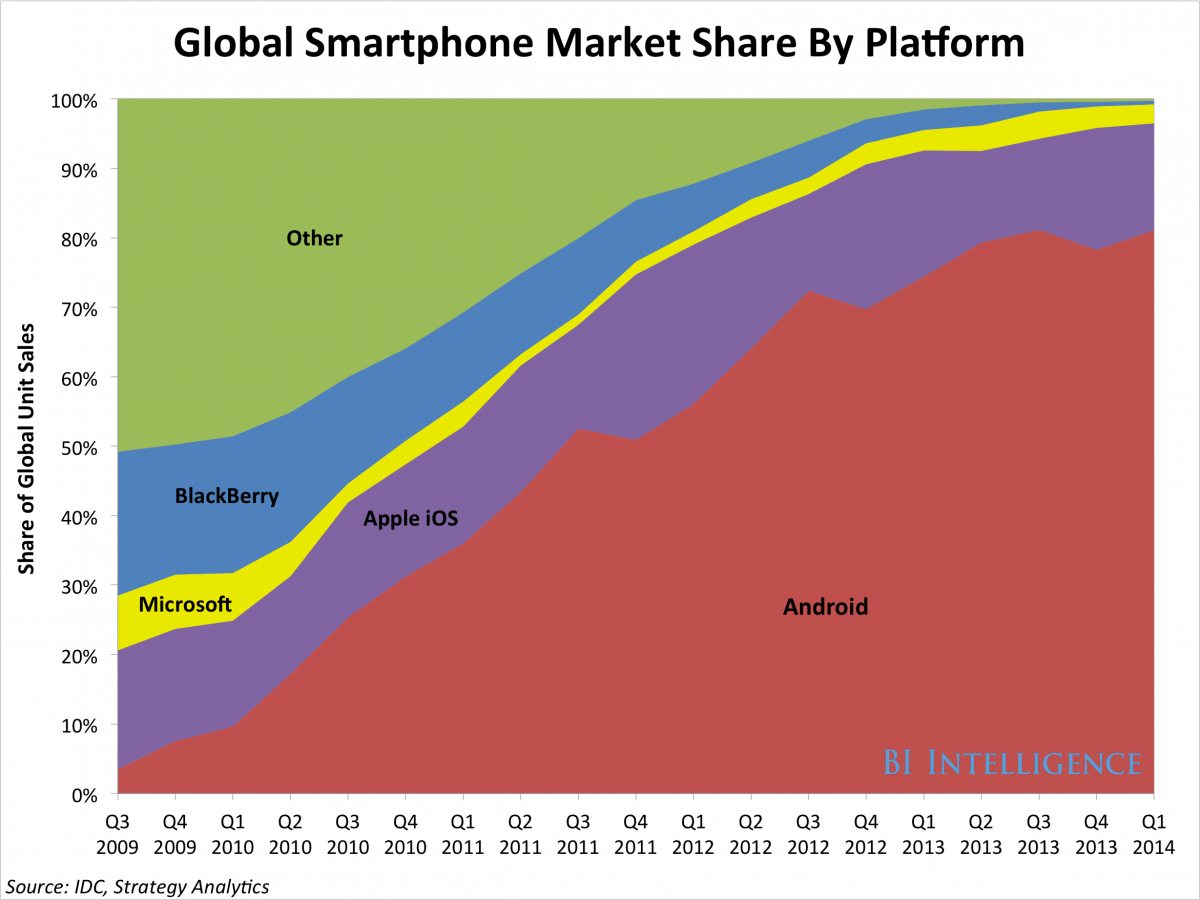
\includegraphics[width=15cm]{images/ProjectComponents/smartphone-market-share.png}
			\caption{Smartphone market share}
			\label{marketshare}
	\end{figure}
	\bigskip


Android has been chosen for the following reasons:
	\begin{itemize}
	\item \textbf{Market share:} Being the operating system used by the highest number of people means that the robot will be useful to the largest amount of users possible.
	\item \textbf{Price ranges:} Because most mobile phone manufacturers nowadays include Android each user will be able to enjoy the product whithout having to pay for a high-end phone.
	\item \textbf{App development:} Finally, Android apps such as Bot Control can be programmed from any computer regardless of the OS, and can be uploaded to the user's phone directly. This means users are able to customize the app with no extra costs, such as having to use a certain OS and paying a developper's fee.
	\end{itemize}


\newpage
In this project a Haipai Noble H686 (Figure \ref{HaipaiNoble}) is used. Some of its more relevant specifications are:
	\begin{itemize}
	\item \textbf{CPU:} Quad-Core Mediatek MTK6589 1.2GHz
	\item \textbf{RAM:} 1 GB
	\item \textbf{OS:} Android 4.2 Jelly Bean
	\item \textbf{Screen Size:} 6.0 inches
	\end{itemize}

	\begin{figure}[H]
			\centering
			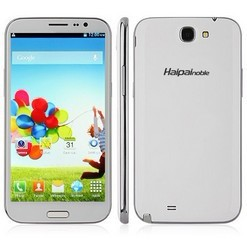
\includegraphics[scale=1]{images/ProjectComponents/android.jpg}
			\caption{Haipai Noble H868}
			\label{HaipaiNoble}
	\end{figure}
	\bigskip

